% 2016 Written PhD Proposal
% Benjamin Rose, advised by Peter Garnavich

%somehow this does not understand \text{}

% \documentclass{aastex}
% \documentclass[preprint2]{aastex}
% default is double spaced `manuscript`, `preprint` or `preprint2` are options
\documentclass[apj, iop]{emulateapj}
\usepackage{graphicx}% Include figure files
\usepackage{color}%for preprints
\usepackage[dvipsnames]{xcolor} %allows for gray links
\usepackage[colorlinks, linkcolor=blue, citecolor=blue, urlcolor=blue]{hyperref}
\usepackage{cleveref} %this allows for \cref{}: http://texblog.org/2013/05/06/cleveref-a-clever-way-to-reference-in-latex/
\usepackage{natbib}
\usepackage{amsmath}  %needed for $\text{}$ and aastex
\usepackage{verbatim}     %for multiline comments with \begin{comment}

\newcommand{\sn}{SNIa}
\newcommand{\todo}[1]{\textbf{\textcolor{red}{#1}}}
\newcommand{\lcdm}{$\Lambda$CDM}     %should use ensure math or something.
\newcommand{\kms}{\ensuremath{~\text{km s}^{-1}}}

% running headers for journal/emulate
\shorttitle{Testing the Cosmological Principle} 
\shortauthors{Rose}

% adds date to aastex versions (emulate has this by default)
% \slugcomment{draft version: \today}
% \slugcomment{}

\begin{document}

\title{Precision Cosmology: Testing the Cosmological Principle \\with Improved Supernova Distances}

\author{Benjamin Rose, {\it advised by} P. M. Garnavich}
\affil{University of Notre Dame, Center for Astrophysics, Notre Dame, IN 46556}
\email{brose3@nd.edu}

% \and
% \author{{\it advised by} P. M. Garnavich}
% \affil{University of Notre Dame, Center for Astrophysics, Notre Dame, IN 46556}

\begin{abstract} 

Type Ia supernova (\sn{}) have become a standard cosmological tool, but there
are still improvements needed in this age of precision cosmology. Cosmology is
reaching a point where we can now start to test the cosmological principle, that
the universe is homogeneous and isotropic on large scales. This is a fundamental
search to validate our understanding of the mass-energy make-up of the universe
and look for entanglement from the era before inflation. I have analyzed the
currently available dataset of \sn{} to search for bulk flows on a variety of
scales. We confirmed a  velocity asymmetries across the sky of $\sim 300~\kms{}$
at low redshift. We cannot rule out a large-scale bulk flow (dark flow) that
could be caused by quantum entanglement in the early universe. And we show that
a larger \sn{} dataset and improved distance precision would provide useful
constraints on any dark flow. LSST will provide a large \sn{} dataset that has
an excellent photometric reliability of $10~\text{millimag}$ across the sky. We plan to
simulate large datasets to determine the optimal observing strategy to constrain
the dark flow given the photometric precision, cadence, and sky coverage
possible from LSST and other \sn{} surveys. Further, we will improve the \sn{}
distance precision by correlating Hubble residuals with properties of the local
environment around the supernova. There appears to be some correlation between
the global host properties (e.g. star formation rate, metallicity) and \sn{}
luminosity residuals. And there is a controversy as to whether the local
environment is biasing the best estimates of the Hubble constant. We will
analyze existing high-resolution Hubble Space Telescope images of SDSS host
galaxies to see if the stellar properties at the explosion location correlate
with \sn{} luminosity.

\begin{comment}
Increasing the precision of \sn{} cosmology allows us to test fundamental
assumptions like the cosmological principle. The objectives of this research are
to continue the analysis of \sn{} calibration and the search of a cosmic-scale
bulk flow. The next step in searching for a cosmic-scale bulk flow is to
simulate and fully understand what is knowable from future surveys like LSST.
The next step for \sn{} calibration is to more fully understand the local
environment. 
\end{comment}

\end{abstract}

\maketitle

\section{Introduction}\label{introduction} 

Type Ia supernova (\sn{}) have been a standard cosmological tool since they were
successfully used to estimate the Hubble constant \citep{Hamuy95,Riess95}, and
later see the accelerated expansion of the Universe
\citep{Riess98,Perlmutter99}. Cosmology is now focusing on precision and with
improved precision we are able to test a fundamental assumption of cosmology:
that the universe is homogeneous and isotropic on the largest scales. In order
to check the Cosmological Principle, both the statistical and systematic
uncertainties in \sn{} distances must be reduced. These measurements will give
deeper understanding of the evolution of the cosmos and the structure and
composition of the universe.

Simple tests can be constructed to see if there is a consistent cosmology in all
directions. For these to reach out to distances of gigaparsecs, or of order
$0.1$ in redshift, \sn{} need to have very accurate distance measurements. \sn{}
distances are already corrected for light curve width and color variations, but
further new corrections appear to be important distance accuracy, such as
correlations with host galaxy properties or even the local environment near the
explosion. Procuring these tests will \todo{finish my thesis statement.}

\section{Testing the Cosmological Principle}\label{testing-the-cosmological-principle}

The excepted cosmological model, $\Lambda$CDM, works under a testable assumption
that the universe is isotropic and homogeneous on large scales, scales greater
than the size of the present day first acoustic peaks seen in the CMB.
%(\cite{Scrimgeour12} says greater-equal 100h$^{-1}$Mpc in ΛCDM).   
We already
know that gravity breaks this isotropic condition on small scales and produces
peculiar motion of galaxies. Specific theories of inflation (like in
\cite{MersiniHoughton:2008io}) produce a preferred direction in our visible
universe due to a slight curvature in space-time from pre-inflation
interactions. \todo{go into theory detail?} Observationally, if this preferred
direction exists, we expect to see a  uniform bulk velocity flow that extends
outside the local group and into what $\Lambda$CDM would predict to be a purely
isotropic Hubble expansion. Such a large-scale asymmetry has been called a `dark
flow'. 
\todo{by whom, Kashlinsky's first paper or his ``review'' paper?}
\todo{define the difference between dark and bulk?}

\subsection{Previous Tests}\label{previous-tests}

The universe's isotropic nature has been tested, over the last decade, with
surveys of nearby galaxies \citep{Ma13}, kinetic Sunyaev-Zel\'{d}ovich (kSZ)
effect on distant clusters \citep{Kashlinsky10,Planckdf}, and with \sn{} data
sets \citep[and others as seen in \Cref{t:review}]{Dai11,Rathaus13}. Most
searches did not see a bulk flow that was significantly larger then allowed by
\lcdm{} but some saw a bulk flow of greater then $1000 \kms{}$ out to
redshifts of $z = 0.25$. This measurement cannot be explained by $\Lambda$CDM
alone but needs an inflation theory that predicts this cosmic anisotropy.  A
summary of the results from past searches can be found in \cref{t:review}.
\todo{remove both table references here.}

\todo{kaslinskly plot of measurements and what LCDM can allow.}

\todo{other plot from aps presentation}

\begin{figure}
	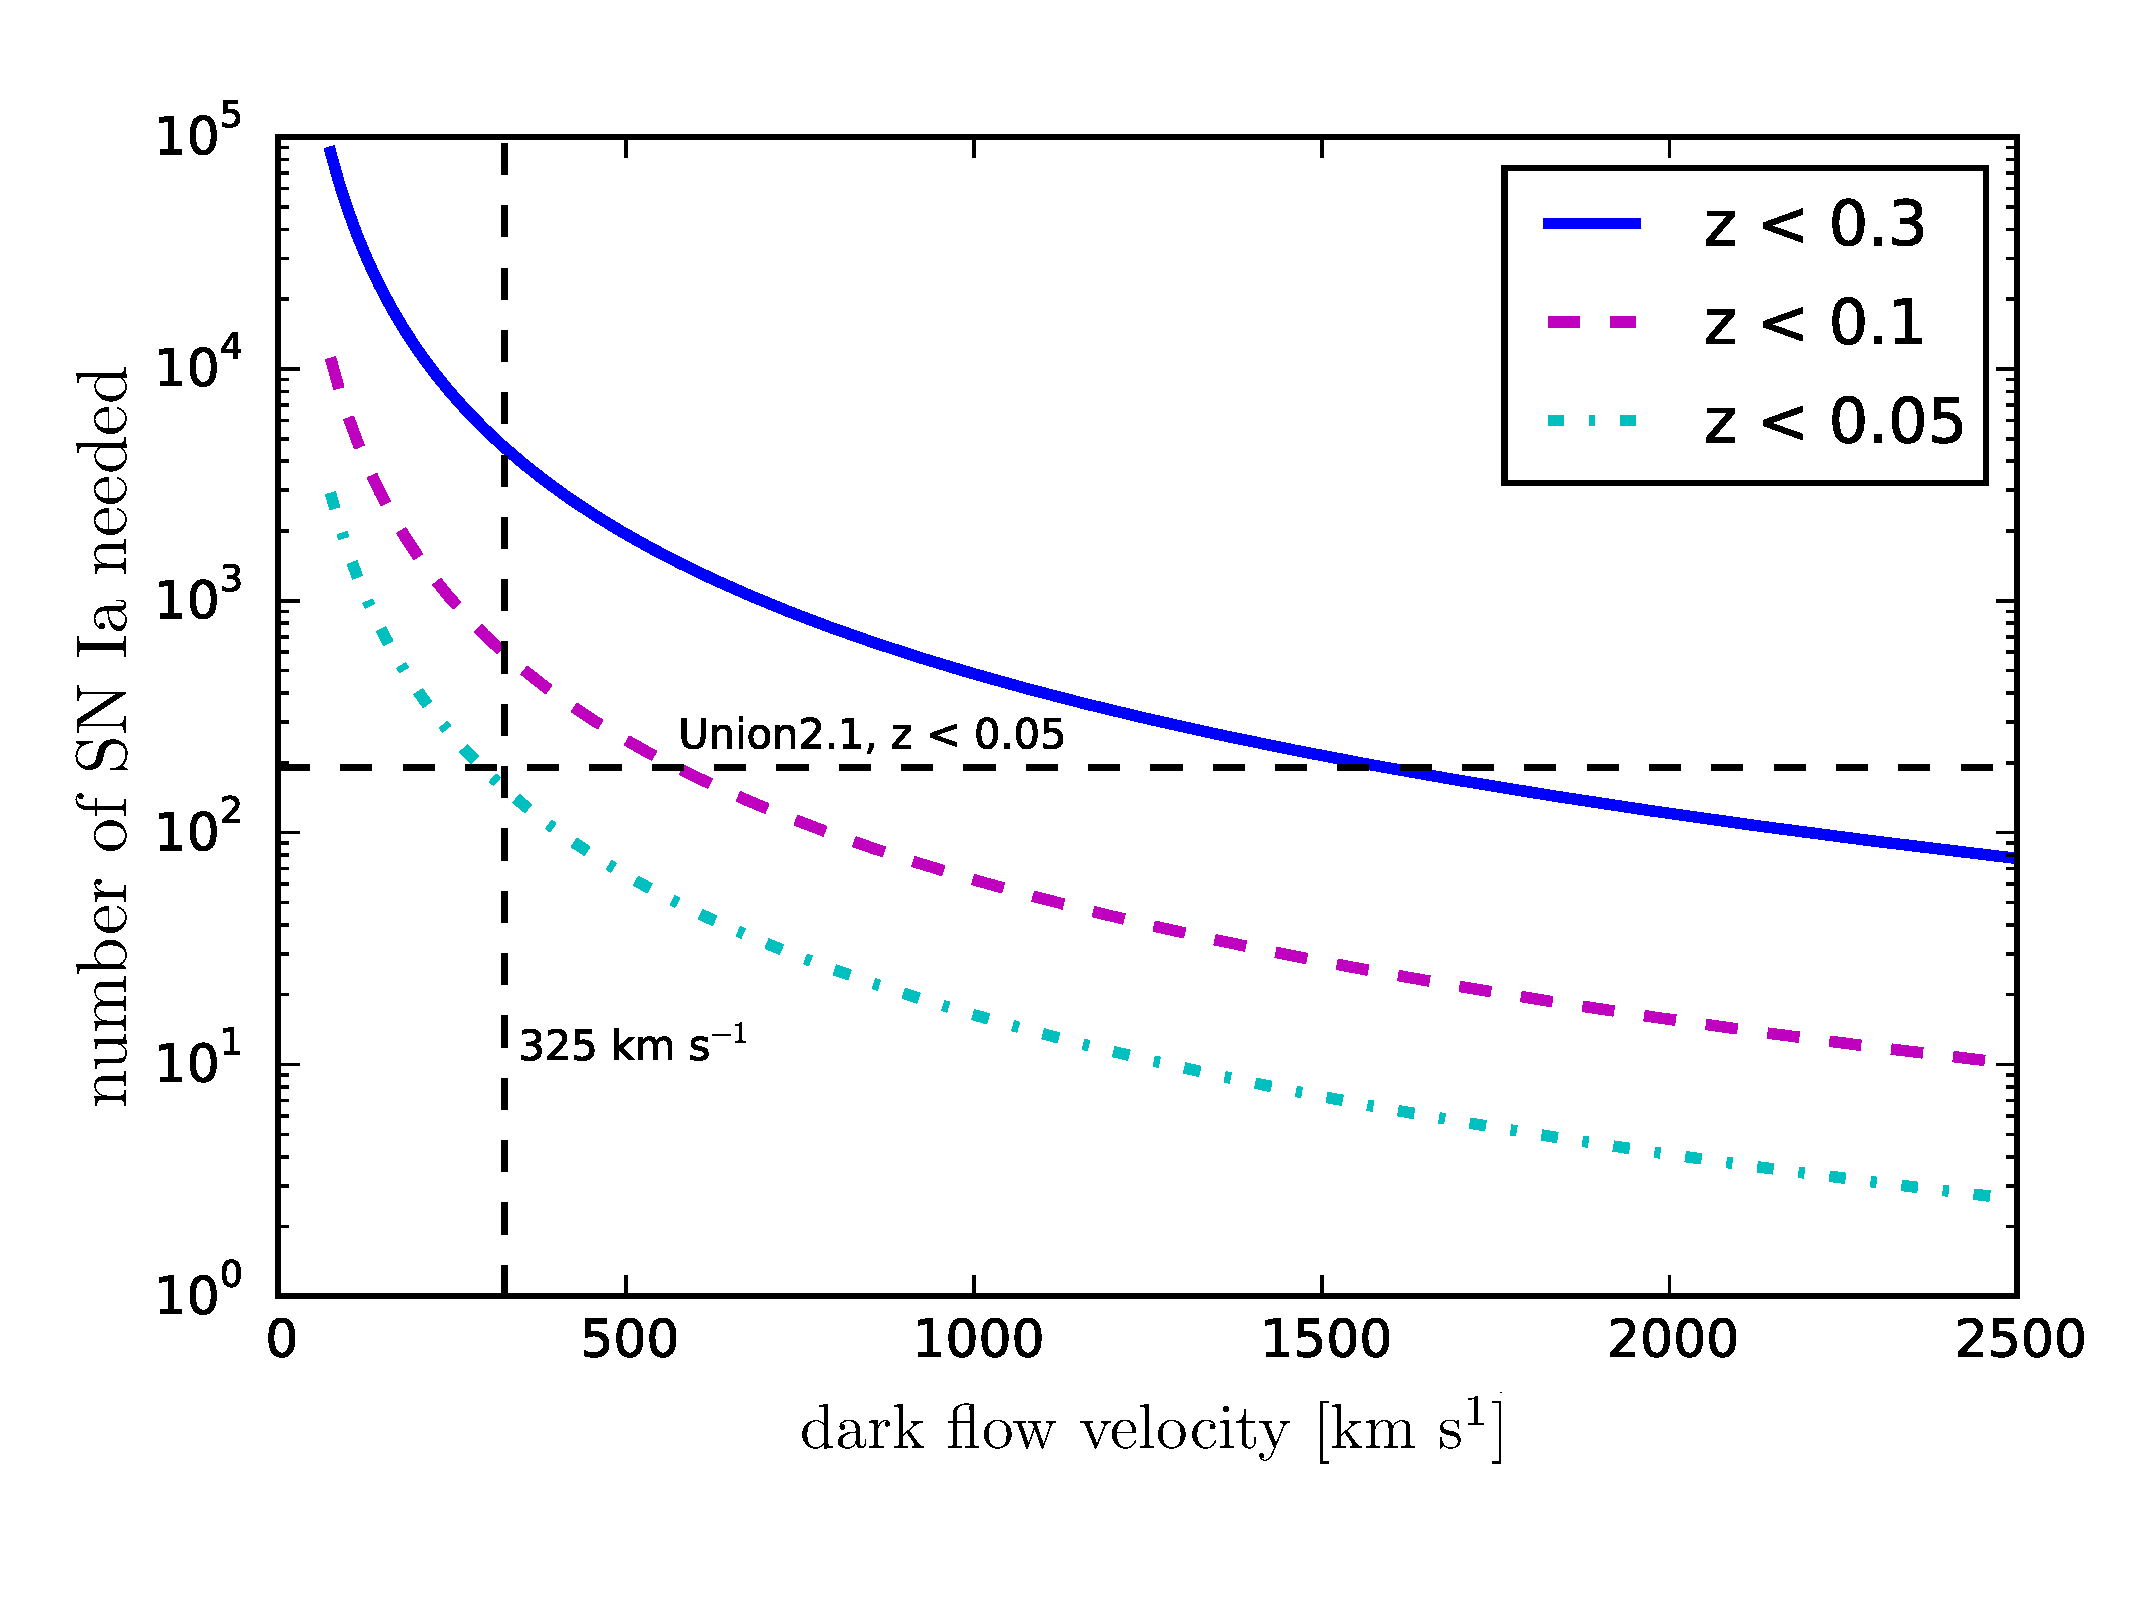
\includegraphics[width=3.2in]{what_dataset_size_v_velocity.pdf} 
    \caption{The number of \sn{} needed to see a given dark flow velocity, a
	cosmic scale bulk flow, out to a given redshift. It is seen that Union2.1 
	can detect flows only out to $z=0.05$ and nearly 10$^4$ \sn{} would be 
	needed to see a dark flow out to $z=0.3$. Taken from \cite{Mathews16}}
	\label{f:sn-needed} 
\end{figure}

My work on initial tests of the Cosmological Principle can be found in
\cite{Mathews16}. I worked heavily on developed a new method to search for
cosmological asymmetries using the angular separation of a \sn{} and the
direction of the dark flow. We were able to minimize the data fitting both
\lcdm{} cosmological variables and  an bulk flow. If the same bulk flow is
visible across all redshifts, then we have found the dark flow signal. This
analysis was performed on the Union2.1 \citep{Suzuki12} \sn{} sample. We found a
mild bulk flow of $325 \pm 54$ km s$^{-1}$ out to $z = 0.05$. This is consistent
with most past measurements and does not contradict \lcdm{}.

From further analysis, we determined that the loss of signal past $z \sim 0.05$
was not from the lack of a dark flow, but from the increase of the uncertainty
in the distance measurements. An order of magnitude reduction of distance
modulus error is needed to see out to $z \sim 0.3$. This is unattainable with
the current data sets, but we propose two ways to attack this problem. First,
further data sets will reduce the statistical error in \sn{} distances over
large parts of the sky. This relationship is illustrated in \cref{f:sn-needed}.
This large sample size should be achievable with the Large Synoptic Survey
Telescope (LSST) and its uniform photometric reliability of $10 ~\text{mmag}$
across the visible sky \citep{Ivezic08}. A large, uniform data set will push the
statistical errors at $z\sim 0.3$ to the systematic floor. Second, we propose to
lower the systematic floor by including the properties of the local host
environment in correcting \sn{} distances.

\subsection{Future Tests}\label{future-tests}

\begin{comment}
Testing the Cosmological Principle can and should be continued. In search for a
cosmic anisotropy, studies have used galactic surveys, the kinetic Sunyaev-
Zel\'dovich effect, and SNIa, but another possibility is using baryon acoustic
oscillations (BAO). This distance measure is complementary to \sn{} estimates
and subject to smaller systematic uncertainties.
The BAO analysis will follow a similar procedure as developed in
\cite{Mathews16} for SNIa. The test requires a
data set with significant sky coverage, and this is possible with SDSS's eBOSS
and eventually DESI.
\todo{This might want to be removed, do I want to open up questions about BAO?}
\end{comment}

At the end of \cite{Mathews16}, we suggest that LSST will produce a data set
that is able to search for the cosmic dark flow. Detailed simulations of LSST-
like data sets are critical in understanding the limits of the survey when
applied to the dark flow problem. These tests will show if the combination of
LSST's sensitivity, cadence, and sky coverage will be sufficient to test for
isotropic expansion as predicted by \lcdm{} and what limits can be placed on the
dark flow. WFIRST may also be able to help in this measurement, however, its sky
coverage will be limited compared with LSST. Simulations of the combined LSST
and WFIRST data sets will produce useful insights into optimum future surveys.

Since the analysis method is written, getting a good simulated LSST \sn{} data
set is the hardest part. Telescope uncertainties and project goals have been
stated, but these need to be transitioned, and any errors propagated, into
positions,  redshifts, and distances. The hardest part will be redshift. The
community will  not be able to get a spectra of the hosts at the rate that LSST
will find \sn,  reducing the rate of cosmologically usable \sn. Also with follow
up telescopes  in different locations then LSST, the footprint of the
cosmologically useful \sn{} might be different then LSST's footprint. These and
others survey complexities  will need to be taken into account for any accurate
modeling of what can be done with LSST \sn{}.

Large surveys are being leveraged to reduce the statistical uncertainties
in distance measurements. But we also plan to reduce the systematic error floor
by studying the local environments of \sn{}.

\todo{talk about difficulties and solutions}

\section{Standardizing type Ia
supernova}\label{standardizing-type-ia-supernova}

The \sn{} community as a whole is focusing on reducing uncertainty in \sn{}
distances. Knowing distance more precisely will narrow the range for the Hubble
constant, the dark energy equation of state as well as constraining the
Cosmological Principle.

\sn{} are not standard candles, but rather standardizeable candles. Since
\cite{Phillips93} there has been significant work to improve off this basic
correction to the variability in \sn{} absolute luminosity. \sn{} color is also
used to standardize \sn{} and this has allowed them to be used for critical
cosmological measurements (\citep{Riess98, Perlmutter99}). Currently well-
studied \sn{} typically have a 15\% error in distance modulus (or 7\% in
distance). So it takes about 50 \sn{} to reduce the statistical error down to a
few percent in brightness, which is near the the systematic floor. This floor
is partly caused by limits on photometric calibration and partly by intrinsic
uncertainties in the supernovae themselves.

\subsection{New Standardizations}\label{new-standardizations}

A significant amount of research time and energy is spent on trying to reduce
the scatter in the absolute magnitude of \sn{}. It has been found that a
reduction in this can be seen if the properties of the \sn{}'s host galaxy are
accounted for. Host mass \citep{Childress13} and host metallicity
\citep{Hayden13} have been seen to reduce this intrinsic scatter.

The idea that these global properties directly effect the \sn{} is a bit of a
stretch, so the community has started to look at the local environment around
the \sn{}. \cite{Rigault13} looked at \sn{} form the Nearby Supernova Factory
and looked at H$_{\alpha}$ within a 1 kpc radius of each \sn{}. They found  a
bias in standardized brightness of the \sn{}. Also \cite{Rigault15, Jones15}
looked at \sn{} in the Constitution sample with host galaxy data from {\it
GALEX} but they disagree on whether there is or is not a bias. Sorting this
controversy out is critical in improving the estimate of the Hubble constant.

\subsection{Getting Closer in with HST}\label{hst}

I am currently working with Hubble Space Telescope (HST) images of host galaxies
of \sn{} found during SDSS-II Supernova Survey. HST's small angular resolution
allows for a much smaller definition of local environment. For a galaxy at $z =
0.1$ HST can get an environment of $\sim$160 pc, verses the 1 kpc that was used
with {\it GALEX} data in \cite{Jones15,Rigault15}. This can be seen in the
comparison between SDSS (having a simpler angular resolution to {\it GALEX}) and
HST images of the host galaxy of SN 2005fw seen in \cref{f:galaxy-compare}.

\begin{figure}
	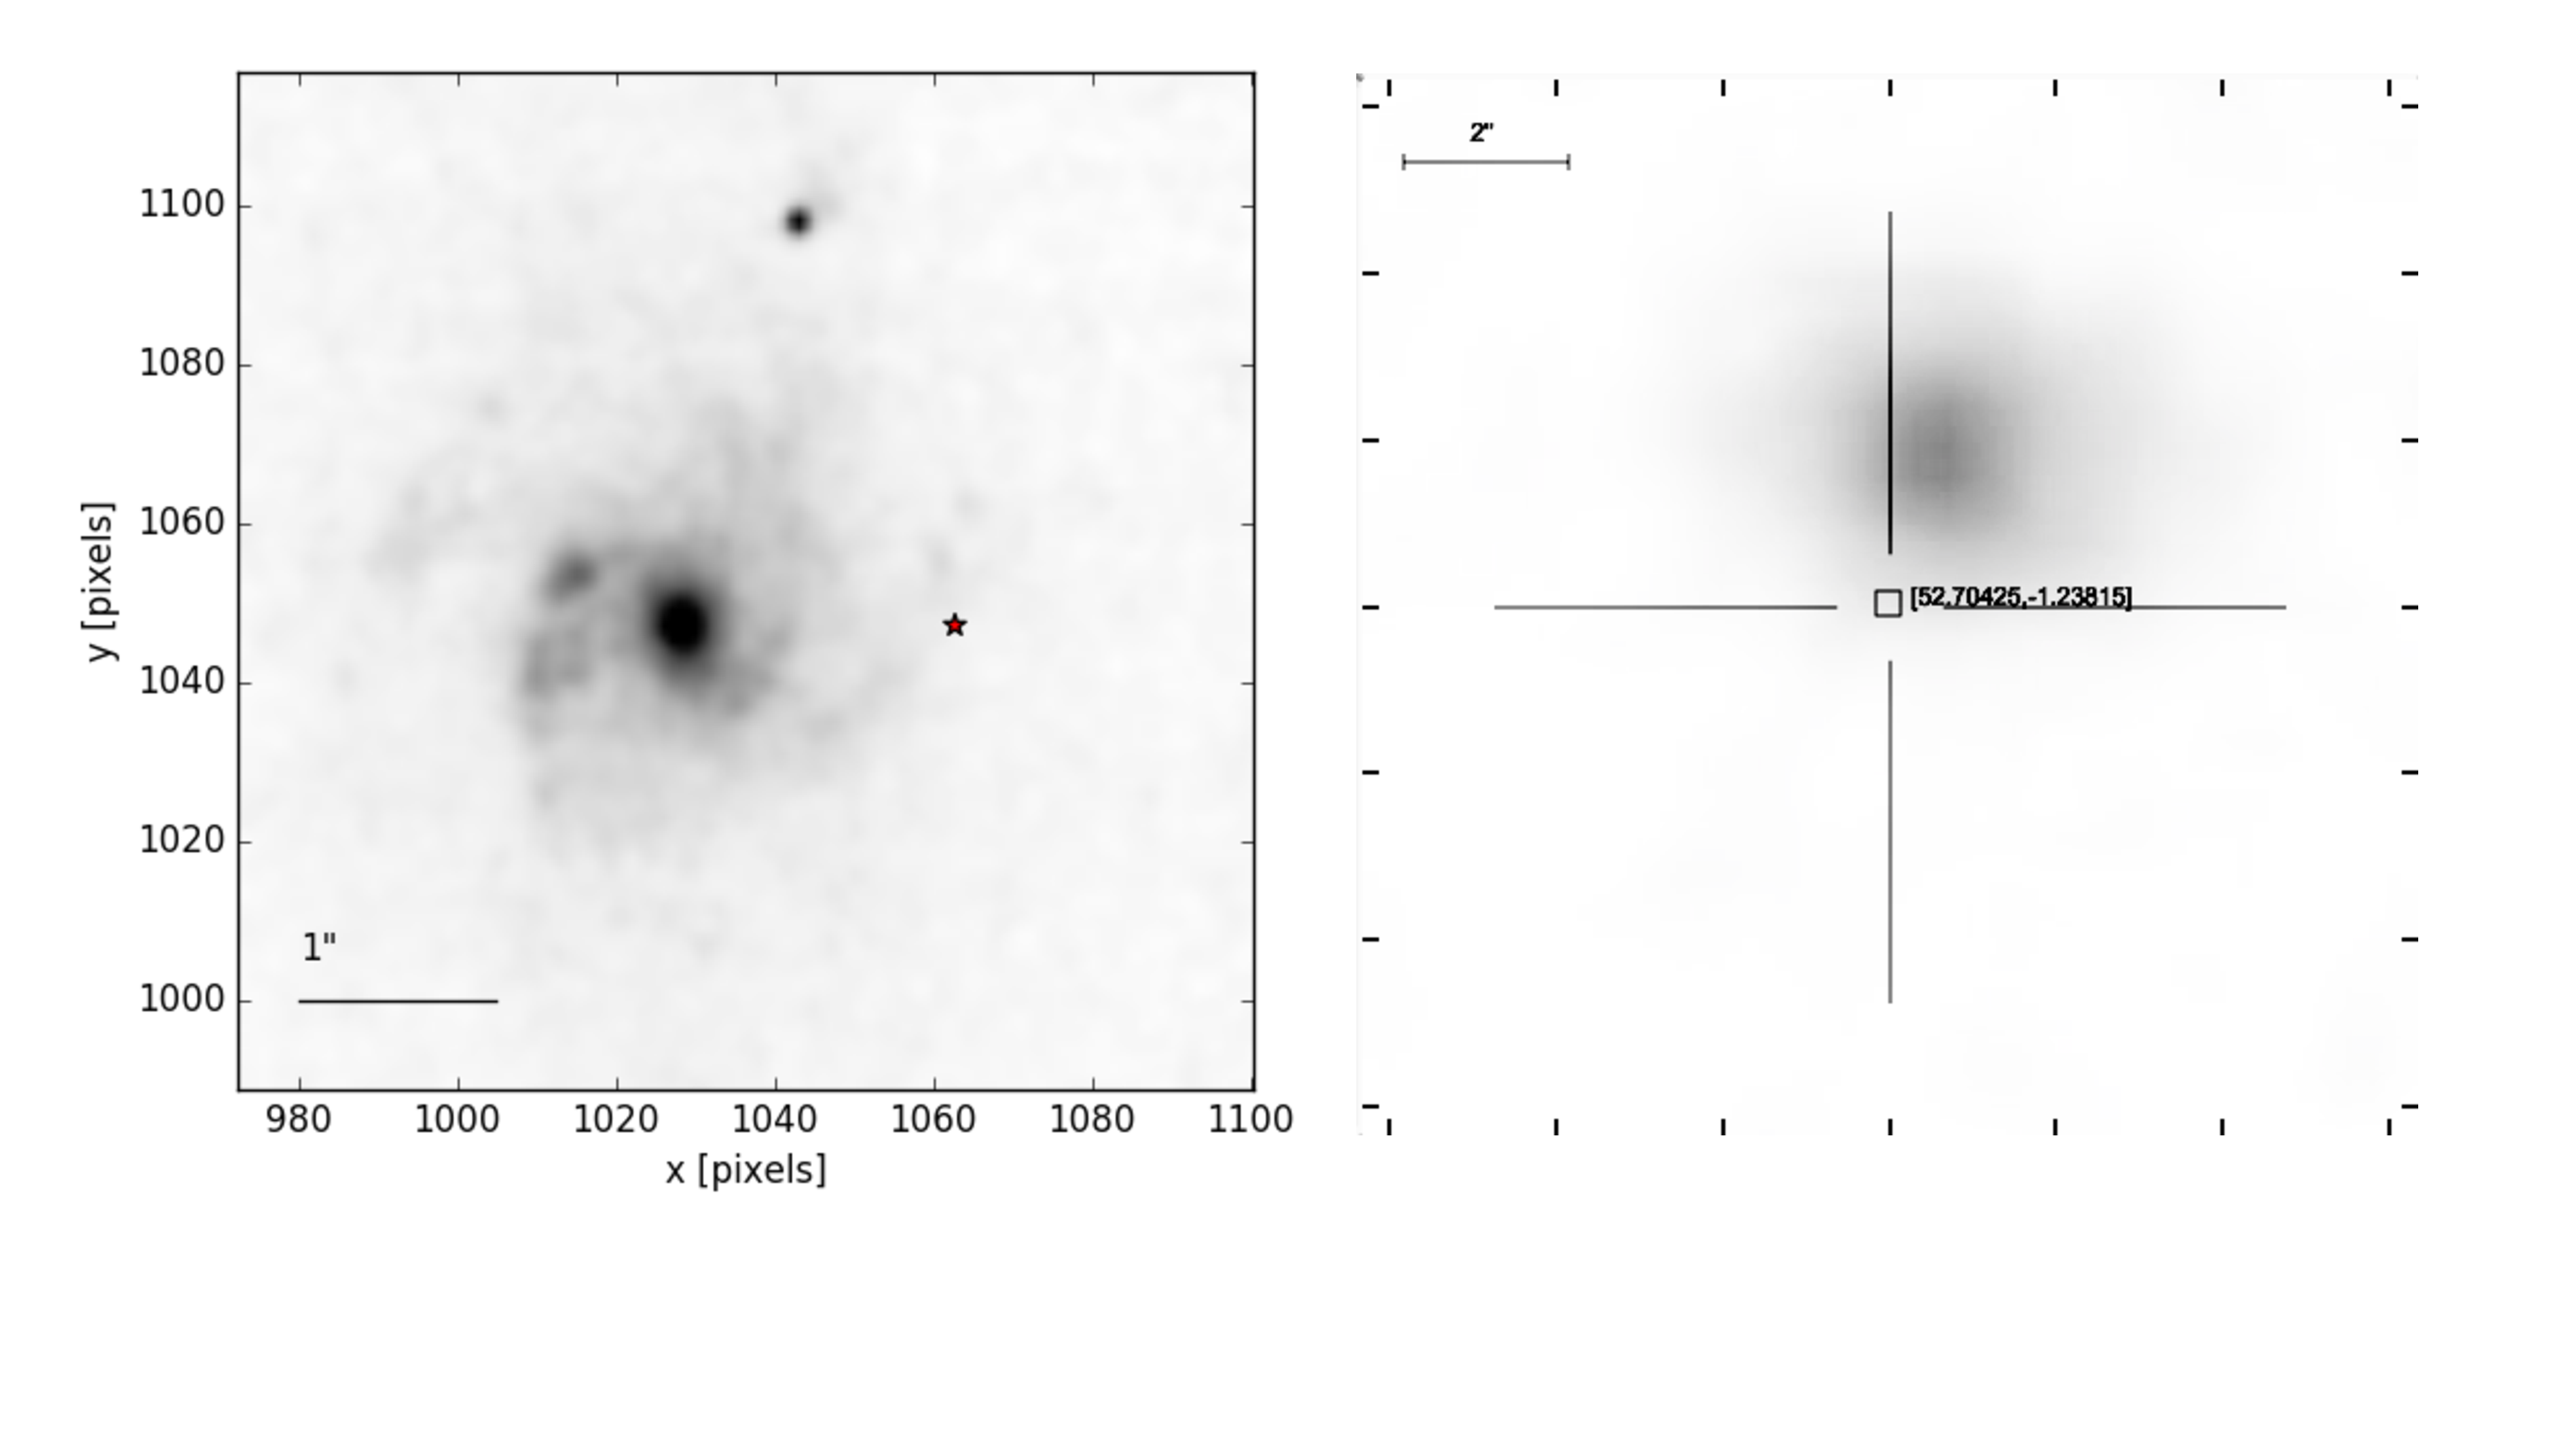
\includegraphics[width=3.2in]{SN2635-combined-inverted.pdf}
	\caption{Host galaxy of SDSS SN2635 (2005fw), at a redshift of z=0.143. HST 
	(left) one pixel is 114 pc, and SDSS (right) one pixel is 1,140 pc.}
	\label{f:galaxy-compare}
\end{figure}

\todo{Describe our HST data. z range, from stripe 82 (elcliptic), filters,
exposure times, angular resolution}

\todo{Take out a few of the instances of ``will.''}
This set of HST images will give us a few variables for the local environment
that we will be able to use for corrections to the \sn{}'s absolute brightness.
The first being the \sn{}'s fractional pixel rank (FPR). The FPR is the ranked
fraction, by brightness, of the pixel at the \sn{}'s position relative to the
rest of the galaxy. This gives us a proxy for star formation. Another variable
would be the color of the \sn{}'s pixel. These two variables will be compared to
the residuals on the Hubble diagram to look for a bias. Further analysis of sub-
sets will be done. We will be able to answer questions like whether there is a
bias for \sn{} in clumpy regions of elliptical galaxies.

% F derivative R - (second derivative) - finds things that do not match 
% its neighbors (nor follows a nice smooth slope like ellipticals)
% a color - Yea color-mag diagram \& ``type/max age'' of stellar region

\subsection{Beyond HST}\label{beyond-hst}

Difficulties in this analysis will all come from the data itself. The most
obvious issue is that there are only 61 host galaxies, compared to around 1000
\sn{} were seen with SDSS \citep{Campbell13}. There is a large number of targets
that still could be observed to increase the data set and improve our
statistical uncertainties. More HST observations would be optimal, because it is
needed for it high angular resolution in the visible. Ground based infrared
photometry with adoptive optics would produce an interesting data set, but it
would be difficult to add it to our current optical data.

We can get more data in several other ways. SDSS-IV's MaNGA is using integrated
field units (IFUs) to get spectra at spacial scales of $\sim 2 ~\text{kpc}$.
IFUs are a common technique and their resolution will only get smaller with
time. Alternative IFU's can be used, including Keck OSIRIS that observes in the
infrared with a spacial element similar to HST ($0.020'' - 0.100''$)
\citep{OSIRIS},
% \url{http://ifs.wikidot.com/instruments#toc12})  
or Gemini GMOS that observes in the optical but has a much larger resolution
$0.2''$ \citep{Gemini}.
% \url{http://ifs.wikidot.com/instruments#toc7}) 

The angular resolution would not be as necessary if we observed host galaxies of
local \sn{}, but local observations also has issues. First, the number of \sn{}
is proportional to the volume for which you are looking, and there is more
volume at higher redshift. Secondly, there are questions about whether \sn{} are
the same across cosmic time \todo{(find citation)}, so these local environment
test should be done for as wide a range of redshifts as possible. For these
reasons, SDSS's $z \sim 0.1$ is a good redshift to perform these tests. At this
redshift, HST's high angular resolution is the best for observing a true local
environment.

\todo{what todo about low s/n? Simulations!}

\section{Conclusion}

\todo{conclusion}


% A slit on the SN location. (idk if this is done, or useful?)

% Ground based observations of hosts

% More HST: filters of these, more statistics, . . .

\bibliographystyle{apj}
\bibliography{2016-02-07-w-ResearchProposal}

\begin{deluxetable}{ccc|cc|c|cc}
\tablecolumns{8}
% \tabletypesize{\small} %equal to title size, seems too big
% \tabletypesize{\footnotesize} %can split after Rathaus13
\tabletypesize{\scriptsize} %one line (+ footnotes) too long for one page
% \tabletypesize{\tiny} %fits on one page
\tablewidth{0pt} %its natural width, (fix different natural widths with info from log file)
% \tablewidth{556pt} %from log tables are 524.95901pt & 555.51466pt wide. But this look strange.
% \rotate
\tablecaption{Summary of bulk flow searches.\label{t:review}} %really a title
\tablehead{
	\colhead{Reference} & \colhead{Obj. Type} & \colhead{No. Obj.} & \colhead{Redshift\tablenotemark{a}} & \colhead{Distance\tablenotemark{a}}  & \colhead{$v_{bf}$} & \colhead{$l$} & \colhead{$b$} \\
	\colhead{}			& \colhead{}		  & \colhead{}		   & \colhead{}		 					 & \colhead{h$^{-1}$ Mpc}				& \colhead{km s$^{-1}$} 	& \colhead{deg}	& \colhead{deg}
	}

\startdata
\cite{Kashlinsky10}  & kSZ & 516 & $< 0.12$ & $< 345$ & $934  \pm 352$ & $282 \pm 34$ &  $22 \pm 20$ \\
                            & & 547 & $< 0.16$ & $< 430$ & $1230 \pm 331$ & $292 \pm 21$ & $27 \pm 15$ \\
                            & & 694 & $< 0.20$ & $< 540$ & $1042 \pm 295$ & $284 \pm 24$ & $30 \pm 16$ \\
                            & & 838 & $< 0.25$ & $< 640$ & $1005 \pm 267$ & $296 \pm 29$ &  $39 \pm 15$ \\ 
\tableline
\cite{Dai11} & SN Ia & 132 & $< 0.05$ & $< 145$ &  $188 \pm 120$  &  $290 \pm 39$ & $20 \pm 32$ \\
                                      & & 425 & $> 0.05$ & $> 145$ &  \nodata     &   \nodata    &   \nodata   \\
\tableline
\cite{Weyant11} & SN Ia & 112 & $< 0.028$ & $< 85 $ & $538 \pm  86$ & $250 \pm 100$ & $36 \pm 11$ \\ 
\tableline
\cite{Ma11}   & \begin{tabular}{c}galaxies \\ \& SN Ia \end{tabular} & 4536 & $< 0.011 $ & $< 33$ &    $340 \pm 130$ & $285 \pm 23 $ &$ 9 \pm 19$ \\ 
\tableline
\cite{Colin11} & SN Ia & 142 & $< 0.06$ & $< 175$ & $260 \pm 130$ & $298 \pm 40 $ &$ 8 \pm 40$ \\
\tableline
\cite{Turnbull12} & SN Ia & 245 & $< 0.05$ & $< 145$ & $245 \pm  76$ & $319 \pm 18 $ &$ 7 \pm 14$ \\ 
\tableline
\cite{Feindt13} & SN Ia  & 128 & 0.015 - 0.035 & 45 -108 & $243 \pm  88$ & $298 \pm 25$ &$15 \pm 20$ \\ 
                                             & & 36  & 0.035 - 0.045 & 108 - 140 & $452 \pm 314$ & $302 \pm 48$ & $ -12 \pm 26$ \\
                                             & & 38  & 0.045 - 0.060 & 140 - 188 & $650 \pm 398$ & $359 \pm 32$ & $ 14 \pm 27$ \\
                                             & & 77  & 0.060 - 0.100 & 188 - 322 & $105 \pm 401$ & $285 \pm 234$ & $ -23 \pm 112$ \\ 
\tableline
% dist is correct, z is a guess
\cite{Ma13}       & galaxies & 2404 & $< 0.026$ & $< 80$ & $280 \pm 8$ & $280 \pm 8 $ &$ 5.1 \pm 6$ \\ 
\tableline
\cite{Rathaus13} & SN Ia & 200 & $< 0.2$ &  $< 550$ & $260$ & $295$ &$ 5$ \\ 
\tableline

% \tablebreak %splits the table over two pages here

%add \citet{Wiltshire13}? & galaxies &
\cite{Appleby14} & SN Ia & 187 & 0.015 - 0.045  & 45 - 130 & \nodata & $276 \pm 29$ &$ 20 \pm 12$ \\ 
\tableline 
\cite{Planckdf} & kSZ &  95 & 0.01 - 0.03 & 30 - 90 & $< 700$ & \nodata & \nodata \\ 
                     & & 1743& $< 0.5$  & $< 2000$ & $< 254$ & \nodata & \nodata\\ 
%Planck number from http://arxiv.org/pdf/1007.1916v1.pdf and from its datafile
\tableline
\cite{Mathews16} & SN Ia & 191 & $< 0.05$ & $<  145$ & $325\pm 54$ & $276 \pm 15$ &$ 37 \pm 13$ \\ 
                                &   & 387 & $> 0.05$ & $> 145$ & $ 460 \pm 260$ & $180 \pm 34$ &$ 65 \pm 340$ \\ 
\enddata

\tablenotetext{a}{Distances and redshifts are either the maximum, or a characteristic value if available from the original source. If distance and redshift were not both given in the literature, calculated distances vs. redshift were done with WMAP parameters: $\Omega_M = 0.288$ and $\Omega_{\Lambda} = 0.712$.}
\end{deluxetable}


\end{document}